\section{Laboratory work implementation}

\subsection{Tasks and Points}
\begin{itemize}
	\item Basic Level (nota 5 || 6):
	
	\item Normal Level (nota 7 || 8):
	
	\item Advanced Level (nota 9 || 10):
	Dezvoltarea unei aplicatii: 
	\begin{itemize}
		\item Desktop
    	\item Mobile	
    	\item Web
    	\item Browser Extension
    	\item Game Development(web,mobile,desktop)
    	\item Service Application
    	\item Internet Application
    	\item Client Application
	\end{itemize}
\end{itemize}
    



\subsection{Analiza lucrarii de laborator}

Linkul la repozitorul Github:\\
\begin{center}
\url{https://github.com/aillyroredshi/MIDPS}
\end{center}

Pentru a realiza acest proiect am utilizat Unity deoarece ne permite posibilitatea de crea aplicatii cross-platform cu usurinta doar avind compnentele necesare instalate pentru platforma dorita.Acest proiect a fost realizat pentru Android si anume Windows(De la versiunea 4.0.1).
\begin{center}
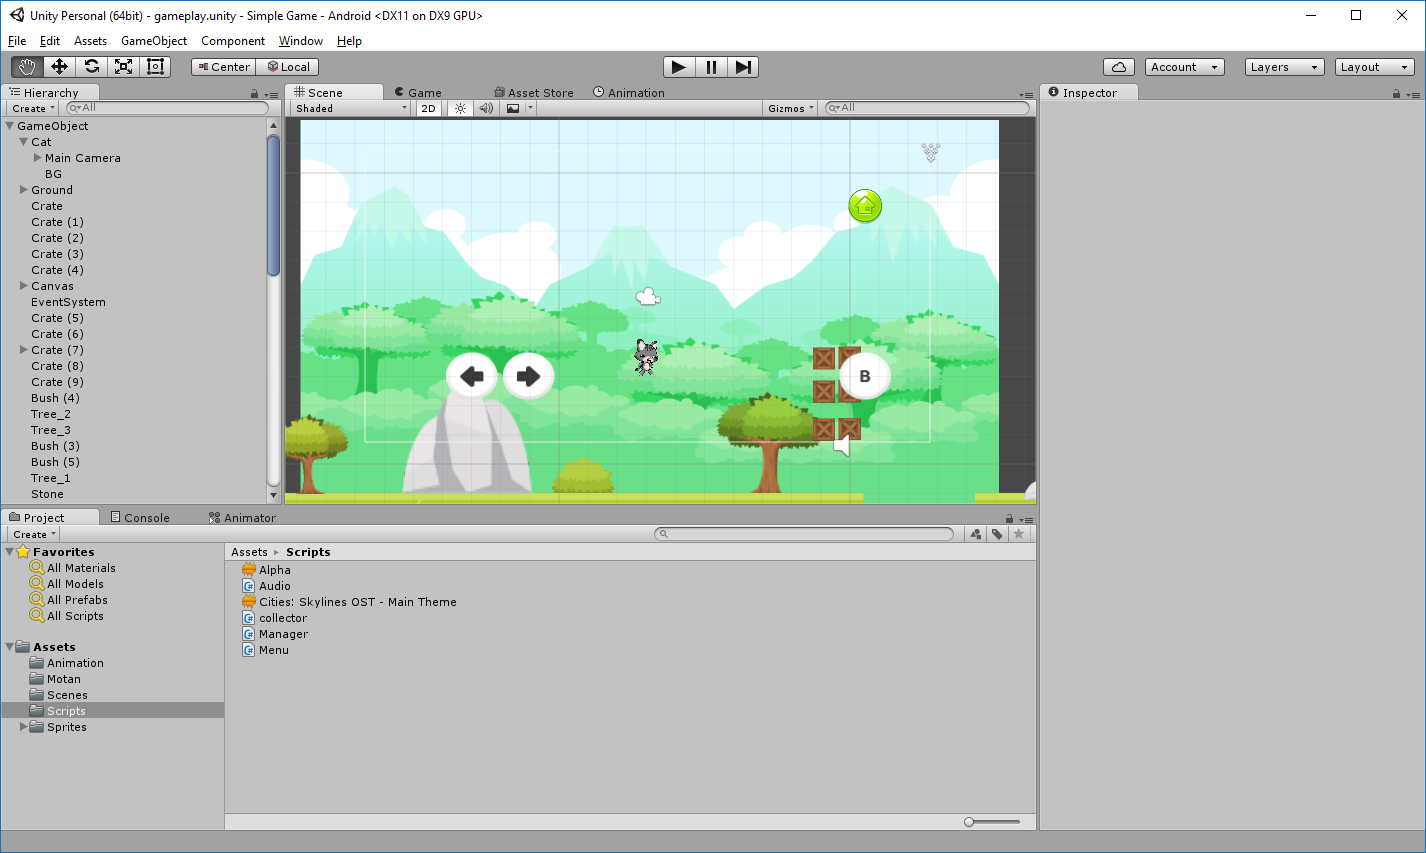
\includegraphics[scale=0.5]{images/1}
\end{center}

Deoarece acest proiect trebuia de realizat in grup ,pentru aceasta ma divizat task-urile in felul urmator:\\

Dupa ce colegul meu a lucrat cu scenele eu am inceput sa lucrez cu scripturile
\begin{center}

\includegraphics[scale=0.5]{images/2}
\end{center}

Pentru a lucra cu scripturi trebuie sa fac animatia la personaj
\begin{center}
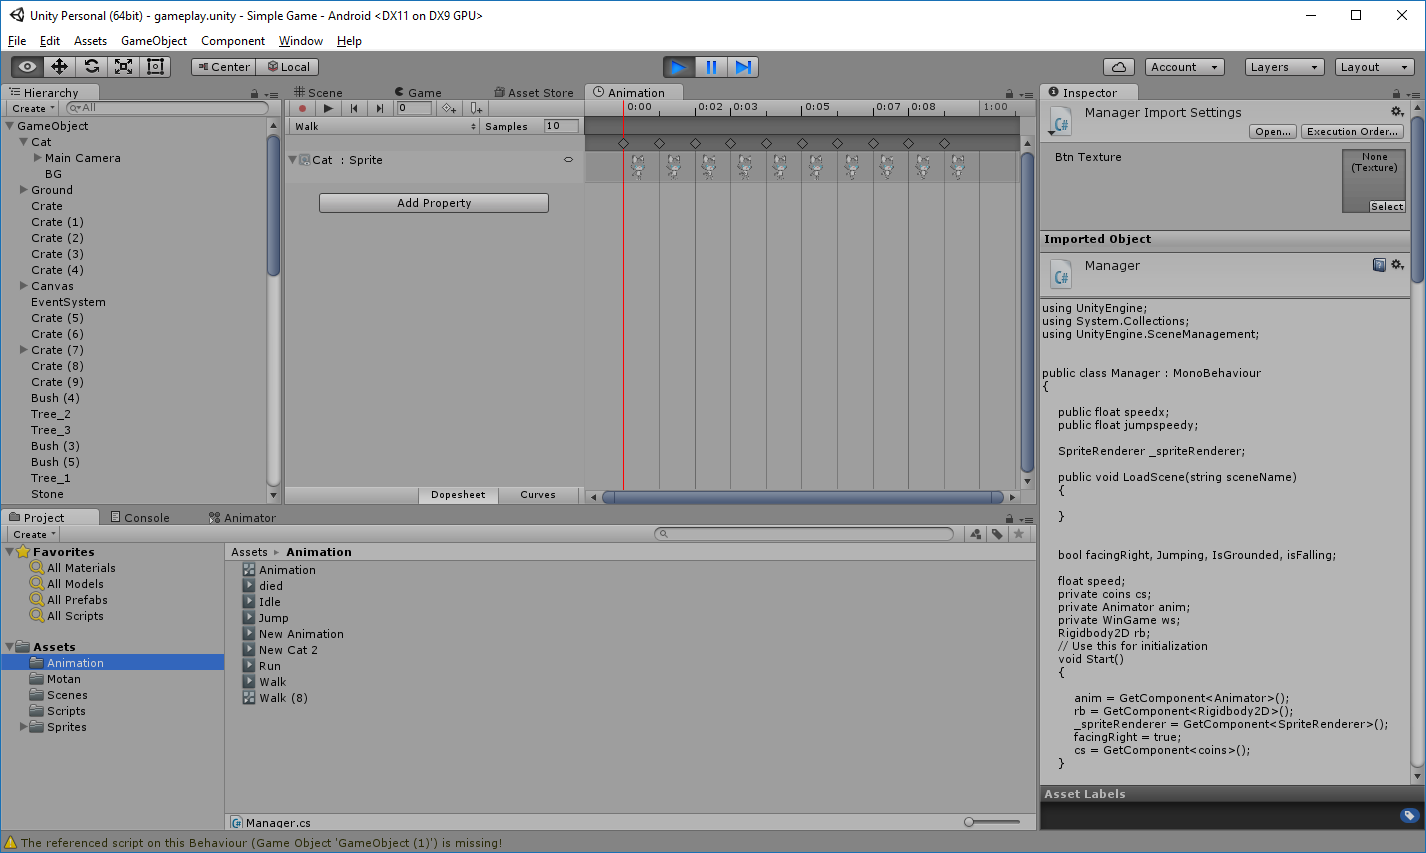
\includegraphics[scale=0.5]{images/3}
\end{center}

Uneste toate animatia pentru a avea o legatura intre dinsele
\begin{center}
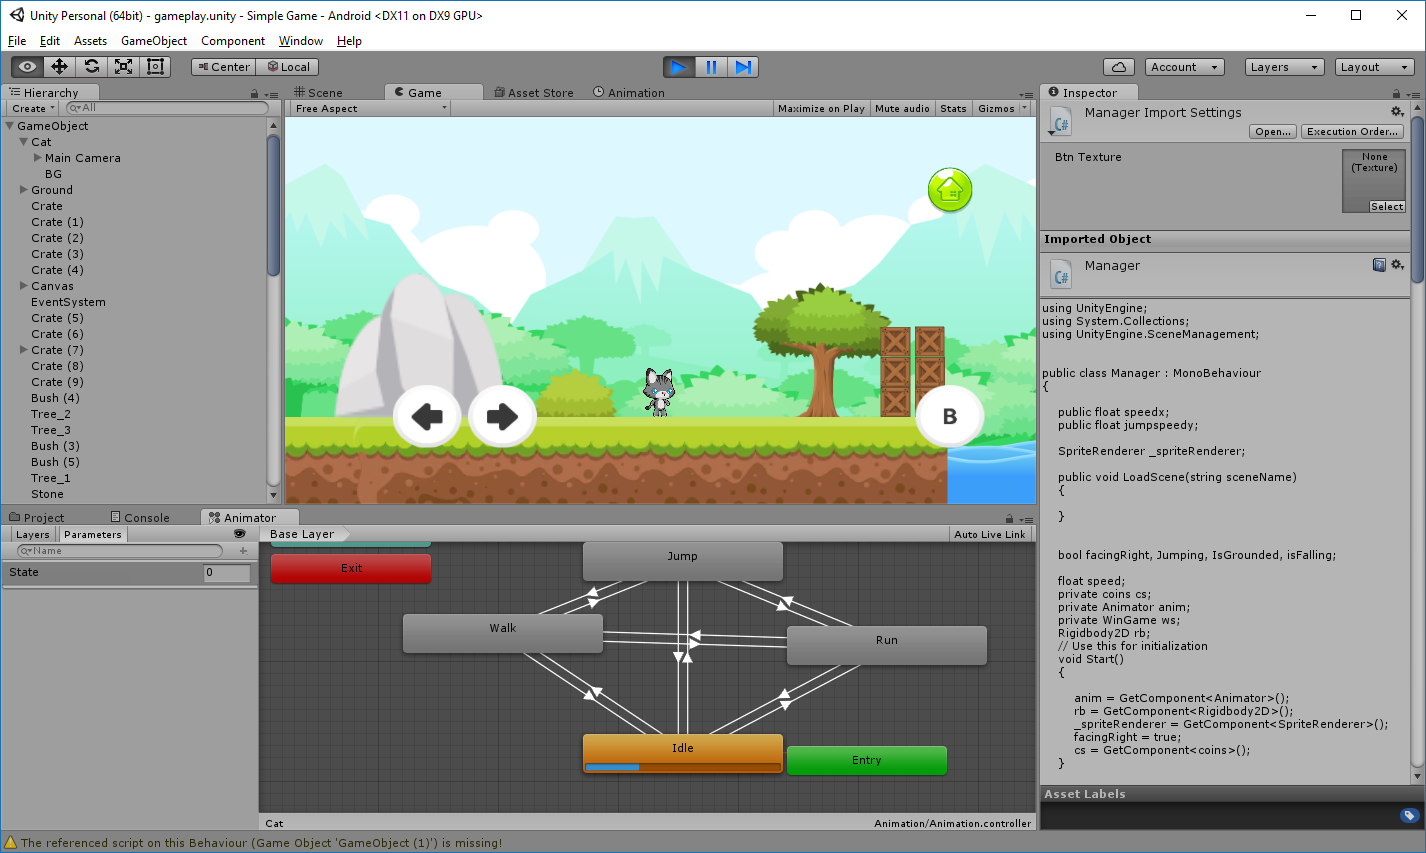
\includegraphics[scale=0.5]{images/4}\\
\end{center}

Pentru a termina cu animatie avem nevoie de a scrie cod pentru miscare  
\begin{center}
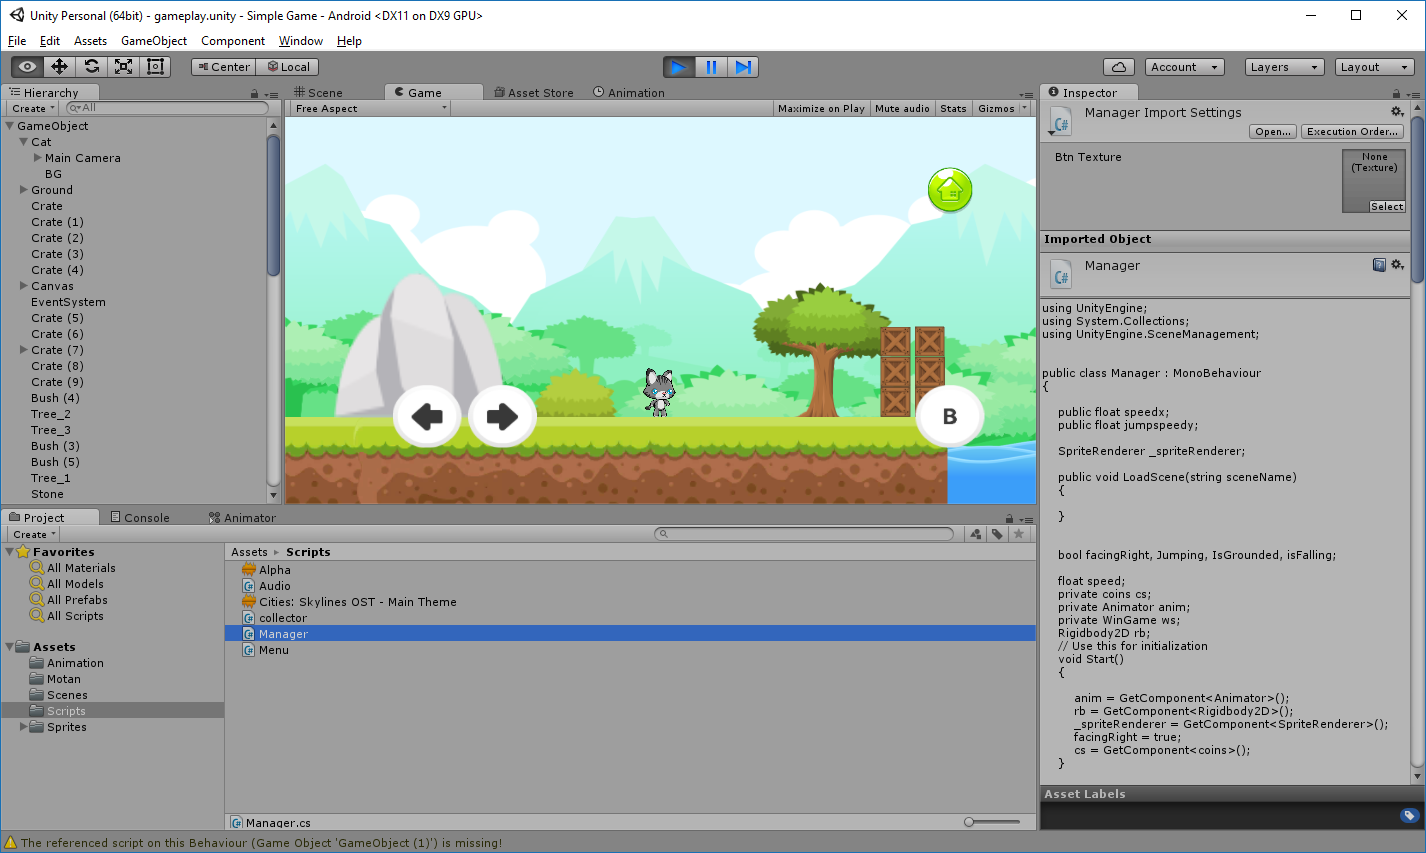
\includegraphics[scale=0.5]{images/5}\\
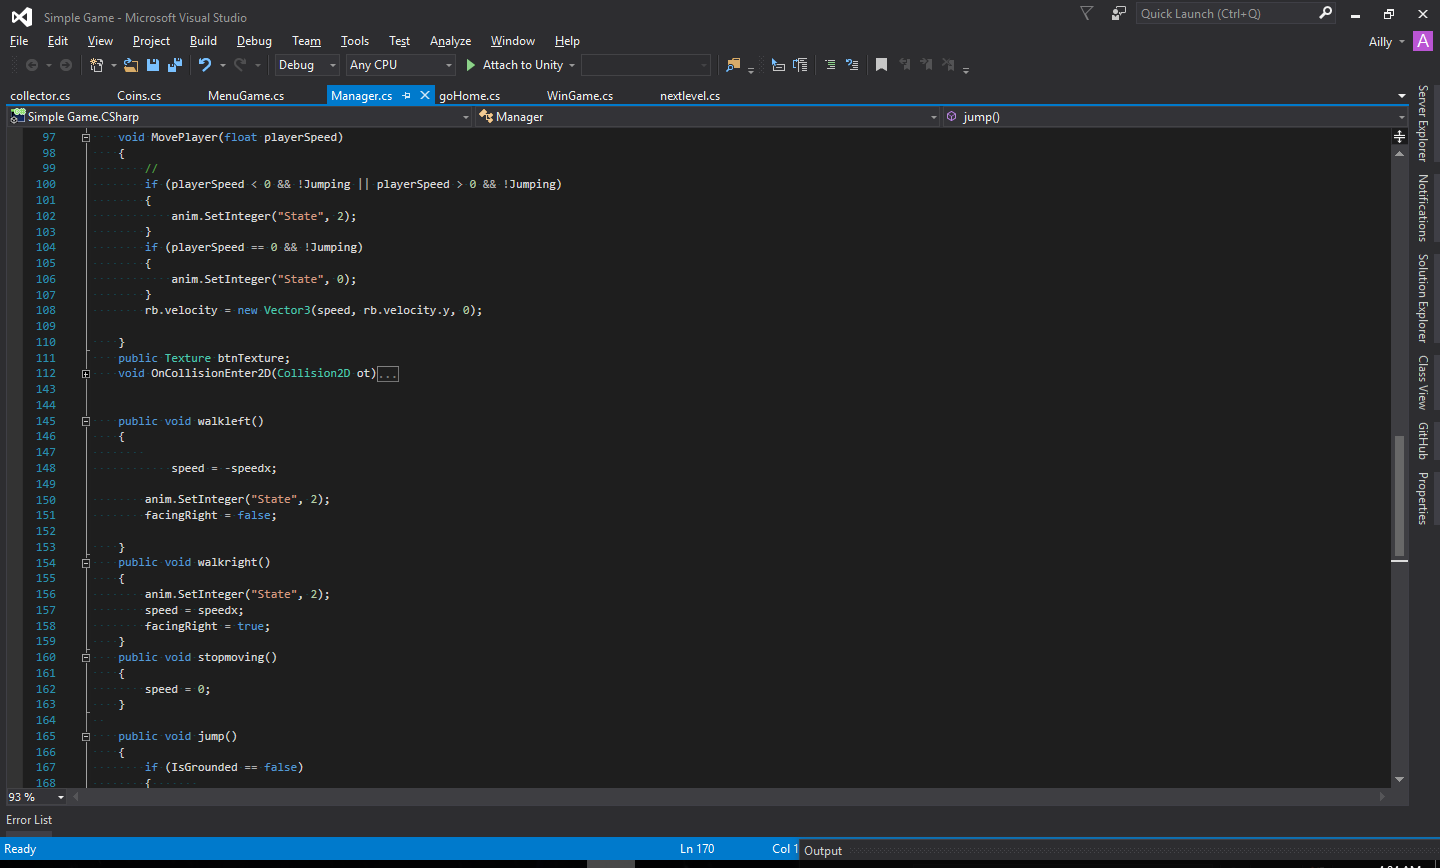
\includegraphics[scale=0.5]{images/6}\\
\end{center}
\clearpage